\begin{figure*}[t]
\begin{center}
\includegraphics[scale=0.35,angle=0]{figures/plotSEDMM18422.eps}
\includegraphics[scale=0.35,angle=0]{figures/plotSEDHLS0.eps}
\includegraphics[scale=0.35,angle=0]{figures/plotSXDF.eps}
\includegraphics[scale=0.35,angle=0]{figures/plotSEDHFLS.eps}
\caption{SED of selected pointlike sources observed with \NIKA\ 2012 and 2013 observation campaigns, 
flux (mJy) as a function of the observed wavelength (mm). 
Upper left : MM18423+5938 observed by \NIKA\ 2012 observation campaign (red points) and previous millimeter observations 
(black points) (\cite{Lestrade:2010wm}). 
Solid line indicates a modified grey body with $\beta=1.5$ and $\rm T=24  \ {\rm K}$, see (\cite{McKean:2011nk}). 
Upper right :  HLSJ091828.6+514223 observed by \NIKA\ 2012 observation campaign (red points) and previous millimeter 
observations (black points), see (\cite{2012A&A...538L...4C}) and references therein. 
Solid line indicates a modified grey body with $\beta=2$ and $\rm T=52  \ {\rm K}$, see 
\citep{2012A&A...538L...4C}.
Lower left : SXDF1100.001 observed by \NIKA\ 2012 observation campaign (red points) and previous millimeter observations  
(black points), see (\cite{Ikarashi:2010ar}) and references therein. 
Solid line indicates a modified grey body with $\beta=1.9$ and $\rm T=20  \ {\rm K}$, see 
\citep{Ikarashi:2010ar}.
Lower right : HFLS3 observed by \NIKA\ 2012 observsation campaign (red points) and previous millimeter observations  (black points), see (\cite{2013Natur.496..329R}) and references therein.}
\label{fig:sedpointlikesources}
\end{center}
\end{figure*} 


\begin{figure*}[t!]
\begin{center}
\includegraphics[height=5cm,width=6cm]{figures/The_Horse_Head_Nebula_1mm.ps} 
\includegraphics[height=5cm,width=6cm]{figures/The_Horse_Head_Nebula_2mm.ps}
\includegraphics[height=5cm,width=6cm]{figures/The_Horse_Head_Nebula_spectrum_map.ps}
%\end{center}
  %\caption{}
%\label{fig:horsehead}
  % \end{figure} 
% \begin{figure}[t!]
%\begin{center}
%\includegraphics[width=6cm]{figures/Cygnus_A_-_Run5_1mm.ps} 
%\includegraphics[width=6cm]{figures/Cygnus_A_-_Run5_2mm.ps}
%\includegraphics[width=6cm]{figures/cygnusa_spectindex.ps}
%\end{center}
  %\caption{}
%\label{fig:cygnusa}
  % \end{figure}  
% \begin{figure}[t!]
%\begin{center}
\includegraphics[width=6cm]{figures/DR21OH_1mm.ps} 
\includegraphics[width=6cm]{figures/DR21OH_2mm.ps}
\includegraphics[width=6cm]{figures/DR21OH_spectrum_map.ps}
\end{center}
  \caption{Examples of 1.25 (left) and 2.14~mm (middle) NIKA maps of well-known extended sources. From top to bottom we present
%the Horsehead nebula, the Cygnus A galaxy including the central source and the hot spots, and the DR21 OH complex. 
the Horsehead nebula and the DR21 OH complex. 
Spectral index maps are presented in the right column.}
\label{fig:extended_sources}
   \end{figure*} 
 
 \begin{table*}
\begin{center}
\begin{tabular}{ccccccccc}
\hline
\hline
Source & RA & DEC  & Integration time   & Noise rms 1.25 mm   &  Noise rms 2.14 mm   & $\tau_{1}$ & $\tau_{2}$ \\
\hline
&  [deg] & [deg] &  [hours] &   [mJy/beam]  &   [mJy/beam]  &  & \\
\hline
Horsehead  &  85.25     &    -2.45  &   1.57 & 14.5  &  2.0   &   0.027 &   0.022 \\
%Cygnus A      &  299.86   &   40.73 &   0.61 &  76.3 & 28.9  &  0.15--0.34 &   0.12--0.33\\
DR 21 OH     &  309.75   &   16.27 &   0.54 & 181.0& 12.6 & 0.27 &  0.22 \\
\hline \hline
\end{tabular}
\end{center}
\caption{Main properties of the maps of extended sources: center of the map, integration time, rms noise, and opacity
at the two observation frequencies.}
\label{tab:extended_sources}
\end{table*}



The \NIKA\ camera was used during the November 2012 and June 2013
campaigns to observe point like sources, in order to assess the \NIKA\
photometry, and extended sources to demonstrate the possibility to reconstruct
angular scales up to few arcminute.


\subsection{Millimeter spectral energy distribution (SED) of selected point sources}
\label{SED}
Point-like sources were observed during the good weather conditions in
the November 2012 and June 2013 campaigns. They were selected to be faint
but detectable, in order to assess the \NIKA\ photometry
with fluxes of a few tens of mJy.
Table~\ref{tab:table_sed} describes the measured point-source fluxes at 1.25
and 2.14~mm. Flux errors are statistical only. The opacity corresponds to a
value averaged over the scans.  Figure~\ref{fig:sedpointlikesources} presents
the spectral energy distribution (SED) of a selection of four sources observed
in the 2012 and 2013 campaigns and compares it with previous measurements. We note
that \NIKA\ observations are in good agreement with previous
observations. We have chosen to observe the following point-source high redshift submillimeter
galaxies (SMG): MM18423+5938, HLSJ091828.6+514223, SXDF1100.001, and HFLS3. For the two campaigns, the weakest source detected
was HFLS3 with a flux of $16\pm 2 \ {\rm mJy}$ at 1.25 mm and $4.0 \pm 0.6 \ {\rm mJy}$ at 2.14~mm.


\subsubsection*{MM18423+5938}
MM18423+5938 is a submillimeter galaxy at $z = 3.93$ discovered
serendipitously (\cite{Lestrade:2009ef}) in a search for cold debris disks
around M dwarfs with MAMBO-2 at the IRAM 30-m millimeter telescope.
  %Although no optical
  %counterpart has been found, J.~-F.~Lestrade {\it et al.} have measured
  %(\cite{} its redshift  from the detection of CO
  %lines using the IRAM Eight MIxer Receiver (EMIR).  
Flux densities at 1.2~mm, 2~mm, and 3~mm were measured
(\cite{Lestrade:2010wm}.  The relatively high flux (about 30~mJy at 1~mm) is
explained by the fact that this SMG is gravitationally lensed, as can be
assessed by the observation of the CO emission, which is consistent with a
complete Einstein ring with a major axis diameter of $1.4^{\prime\prime}$
(\cite{Lestrade:2011qq}.  
Figure~\ref{fig:sedpointlikesources} (upper left) presents the SED of
MM18423+5938 with NIKA measurements and previous ones \citep{Lestrade:2010wm}. J.~P.~McKean {\it et al.}  have fitted the SED with a
single temperature modified blackbody spectrum, with $\beta=1.5\pm 0.5$ and
$\rm T=24^{+7}_{-5} \ {\rm K}$, although the lack of measurements at high
frequencies allows for a wider range of temperatures (\cite{McKean:2011nk}. 
Since NIKA data are not included in the fit, we use it to assess the NIKA photometry. It is presented as a solid line 
in figure~\ref{fig:sedpointlikesources} (upper left).


%The source
%has been measured during the 2013 campaign as well showing the same flux at 2~mm within $2\,\sigma$. The
%discrepancy at 1~mm is likely due to the different bandpasses and the mediocre
%weather at the time of the observations. We suspect that anomalous refraction (\cite{1987A&A...184..381A}) caused significant broadening of the effective beams, diluting the measured flux during this time. 

\subsubsection*{HLSJ091828.6+514223} 
HLSJ091828.6+514223 is an exceptionnally bright source at millimeter and submillimeter wavelength, discovered
behind the z=0.22 cluster Abell 773 (\cite{2012A&A...538L...4C}). It appears to
be a strongly lensed submillimeter galaxy (SMG) at a redshift of z=5.24, the
lens being an optical source lying in the neighborhood. It has been measured
at 2\,mm (IRAM-30\,m EMIR), 1.3\,mm (SMA), and 0.88 mm (SMA) (see
\cite{2012A&A...538L...4C} and references
therein). Figure~\ref{fig:sedpointlikesources} (upper right) presents the SED
of HLSJ091828.6+514223 with \NIKA\ measurements and previous ones \citep{2012A&A...538L...4C}).
F. Combes {\it et al.}  have fitted the SED with a
single temperature modified blackbody spectrum with $\beta=2$ and
$\rm T=52 \ {\rm K}$.
As NIKA data are not included in the fit, we use it to assess the NIKA photometry. The SED is presented as a solid line 
in figure~\ref{fig:sedpointlikesources} (upper right).



\subsubsection*{SXDF1100.001}
SXDF1100.001 (also known as Orochi) is an extremely bright (50 mJy at 1 mm)
submillimeter galaxy, discovered in 1.1\,mm observations of the
Subaru/XMM-Newton Deep Field using AzTEC on ASTE (\cite{Ikarashi:2010ar}).  It
is believed to be a lensed, optically dark SMG lying at z=3.4 behind a
foreground, optically visible (but red) galaxy at z=1.4.\\
Continuum flux densities at millimeter wavelengths have been measured by SMA,
Carma, Z-SPEC/CSO, and AzTEC/ASTE (see \cite{Ikarashi:2010ar} and references
therein). Figure~\ref{fig:sedpointlikesources} (lower left) presents the SED
of SXDF1100.001 with \NIKA\ measurements. To our knowledge, this is the first
measurement at    2\,mm.
S. Ikarashi {\it et al.}  have fitted the SED with a
single-temperature, modified blackbody spectrum, with $\beta=1.9$ and
$\rm T=20 \ {\rm K}$ \citep{Ikarashi:2010ar}.
As NIKA data are not included in the fit, we use it to assess the NIKA photometry. It is presented as a solid line 
in figure~\ref{fig:sedpointlikesources} (lower right).
 


\subsubsection*{HFLS3}
HFLS3 has been reported as a massive starburst galaxy at redshift 6.34
(\cite{2013Natur.496..329R}).  Continuum emission has been measured over a broad
wavelength range, in particular at millimeter wavelengths (Z-Spec, PdBI/IRAM,
CARMA/Caltech, Gismo/IRAM-30m) (see \cite{2013Natur.496..329R} and references
therein). Figure~\ref{fig:sedpointlikesources} (lower right) presents the SED
of HFLS3 with \NIKA\ measurements, which are in good agreement.


\subsubsection*{Other observations} 
These four comparisons of \NIKA\ observations at 1 and 2~mm with previous
observations allow us to assess the NIKA photometry.  Other observations
(shown in the lower part of Table~\ref{tab:table_sed}) allow probing the
diversity of sources and fluxes and measuring the camera performance in various
background conditions. In particular,  Arp220 (aka IC 4553) is the closest (z = 0.018) ultraluminous
infrared galaxy, known to be a merger system composed of a double nucleus. 
Continuum flux densities at millimeter wavelengths has been measured \citep{Sakamoto, Scoville, woody} 
but particular attention must be paid to line contamination due to the prolific molecular line emission. 
S.~Martin {\it et al.} have shown  that 
the contamination of molecular emission to the flux 
constitutes 28~\% of the overall flux between 203 and
241~GHz  \citep{Martin:2010gg}.\\  
HAT084933, HAT133008, PSS2322+1944, and 4C05.19 are high-redshift
point sources. GRB121123A is a gamma-ray burst that happened during the 2012
campaign. ZZTauIRS and CXTau are stars detected by Herschel.


 \begin{table*}[t!]
\begin{center}
\begin{tabular}{ccc}
\hline
\hline
{\bfseries Array} & 1.25~mm & 2.14~mm  \\
\hline \hline
{\bfseries Valid pixels} & 80~(run5)~190~(run6) & 100~(run5)~125~(run6) \\
{\bfseries Field of view}~(arcmin) & 2.2 & 2.2 \\
{\bfseries Band-pass}~(GHz) & 125-175   & 200-280~(run5)~200-270~(run6)  \\
{\bfseries FWHM}~(arcsec) &  12.3  & 18.1 \\
{\bfseries Sensitivity}~(mJy$\cdot s^\frac{1}{2}$) & 40 & 14  \\
{\bfseries Mapping speed}~(arcmin$^2$/mJy$^2$/hour) & 8 & 57  \\
\hline \hline
\end{tabular}
\end{center}
\caption{Summary of the NIKA characteristics and performance. Observation campaign 2012 is referred to as run5. Observation campaign 2013 is referred to as run6}
\label{tab:table_fin}
\end{table*}



\subsection{Mapping of extended sources}   
\label{ES}

During the 2012 and 2013 observation campaigns we observed several well-known extended sources simultaneously at 1 and 2~mm to test the capabilities of
the \NIKA\ camera to recover large angular scales up to few arcmin. We performed
both elevation and azimuth raster scans to ensure an homogeneous coverage of
the mapped area. The size of the scans and integration time have been adapted
to each source. We present two examples of extended sources, namely the
%Horsehead Nebula, the Cygnus A and DR21 OH regions that have been observed
Horsehead Nebula and DR21 OH regions that have been observed
during the 2012 campaign. The center pointing position, the size of the scans,
and the integration time for each sources are given in
Table~\ref{tab:extended_sources}. We also present the median rms of the map
and atmospheric opacity for the 1.25 and 2.14~mm maps.
 
 
\subsubsection*{The Horsehead nebula}
The Horsehead nebula is a dark protrusion that emerges from the L1630 cloud in the Orion B molecular complex at about 400~pc. This condensation is illuminated by the 09.5~V star $\sigma$Ori which is at a distance of 0.5$^{\circ}$ from the cloud. It presents a photon-dominated region (PDR) on its western side, which is seen edge-on  \citep{2003A&A...410..577A}. 

We concentrate here on the outer neck \citep{2005A&A...440..909H}, which
consists of the PDR, the nose, the mane and the jaw. In the top row of
Figure~\ref{fig:extended_sources}, we show the 1.25 (left) and 2.14 (middle)~mm
NIKA maps. The typical one-sigma error in the map with the pixel size of 3 arcsec is 14.5~mJy/beam at 1.25~mm and 2 at 2.14~mm.  The NIKA 1.25~mm is consistent with the
1.2\,mm continuum map \citep{2005A&A...440..909H} obtained with MAMBO2, the
MPIfR 117-channel bolometer array from 30~m IRAM telescope \citep{1992ESASP.356..207K}. In the NIKA maps we clearly
observe the PDR region whose morphology changes significantly
from one frequency to another. This is also obvious in the spectral index map
presented in the right hand figure that ranges between 2 and 5. The northern part of the PDR presents a
significantly flatter spectral index (about 4.5) than the southern part and
the mane (about 3.5). Two possible explanations are CO 2-1 contamination at 1
mm or high dust emissivity spectral index\citep{2013ApJ}. 

%There is also additional evidence of 2 mm emission only that might be due to free-free emission.

%\subsubsection*{Cygnus A}
%Cygnus A is  the most powerful Fanaroff- Riley II (FRII) radio galaxy in the local environment.
%It has been well studied in terms of spatial resolution as it lies
%at a distance of 227 Mpc. The global properties of the object are 
%reviewed in the literature \citep{1996cyga.book.....C}.  At low radio frequencies, the synchrotron emission 
%from the two giant lobes dominate \citep{1974MNRAS.166..305H}. At higher frequencies the
%hotspots (working surfaces in the lobes) and the galaxy core become more prominent.
%The southern and northern hotspots are respectively 50 and 70 arcsec from the core.

%The NIKA maps of Cygnus A at 1.25 (left) and 2.14 (middle) mm are presented in
%the middle row of Figure~\ref{fig:extended_sources}.  The typical rms of the
%map is 76 and 29 mJy/beam at 1.25 and 2.14 mm, respectively.  As expected, the
%two hot spots and the galaxy core dominate the signal at the NIKA
%frequencies. The hot spots present a spectral index (right map on the row) in
%the range -1.5 to -2.0, which is consistent with synchrotron emission but
%steeper than the value found by \citet{1998MNRAS.301..935R}, which is $\sim
%-1$. The galaxy core shows a flatter spectrum from -0.6 to -1.0, which is
%consistent with previous estimates from \citet{1999IAUS..194..179L}.


\subsubsection*{DR21 complex}
DR21 is a giant star-forming complex located in the constellation Cygnus
$\sim 3$ kpc from Earth \citep{1982ApJ...261..550C, DR21_2, DR21_1}.  H2O masers
\citep{1977A&AS...30..145G} and a map of the 1.3-mm continuum emission
\citep{2005IAUS..227..151M} show that DR21 belongs to a north-south oriented
chain of massive star forming complexes. DR21 is composed from north to south
of three main regions DR21, DR21 OH, and DR21 Main (DR21M). DR21M has a mass of
$\sim$ 20000 M$\sun$ and contains one of the most energetic star forming
outflows detected to date \citep{1991ApJ...366..474G,1991ApJ...374..540G,1992ApJ...392..602G}.

We present in the bottom row of Figure~\ref{fig:extended_sources} the NIKA
maps of the DR21 complex at 1.25 (left) and 2.14 (right)~mm. We observe in
them the three main regions in the complex, the most intense being DR21OH and
DR21M. As shown in the right hand plot of the row, the spectral characteristics of
these two regions are significantly different. DR21M has a flatter spectrum in
the frequency range of NIKA.  We suspect the presence of strong free-free
emission.




